\documentclass[envcountsect]{llncs}
\title{Attacks on Search-RLWE}
%\author{Hao Chen, Kristin Lauter, and Katherine E. Stange}

\usepackage{macros}
\usepackage{float}
\usepackage{url}
\usepackage{placeins}
\usepackage{hyperref}
\setlength{\tabcolsep}{7pt}

\spnewtheorem{fact}{Fact}{\bfseries}{\rmfamily}


\usepackage{algpseudocode}
\usepackage{algorithmicx}
\usepackage{algorithm}
\renewcommand{\algorithmicrequire}{\textbf{Input:}}
\renewcommand{\algorithmicensure}{\textbf{Output:}}
%\usepackage{physics}


%%%%%%%%%%%%%% To do notes, can remove later
\usepackage[textwidth=50,textsize=tiny]{todonotes}
\setlength{\marginparwidth}{2cm}
\newcommand{\tinytodo}[2][]
{\todo[caption={#2}, #1]{\renewcommand{\baselinestretch}{0.5}\selectfont#2\par}}
\newcommand{\Katetodo}[1]{\tinytodo[color=green!20]{#1}}
\newcommand{\Haotodo}[1]{\tinytodo[color=red!20]{#1}}
\newcommand{\Kristintodo}[1]{\tinytodo[color=blue!20]{#1}}
%%%%%%%%%%%%%%%%%%%%

\begin{document}
\maketitle

\begin{abstract}
We describe a new attack on the Ring learning-with-errors (RLWE) problem based on the chi-square statistical test, and give examples of Galois number fields vulnerable to our attack. We then analyze the security of cyclotomic fields against our attack.

%Also, we sharpen the attack in \cite{elos2015weak} and give examples of vulnerable instnaces of cryptographic size. Finally, we discuss the effect of modulus switching on our attacks.
\end{abstract}

\section{Introduction}
The Ring Learning-with-Errors (RLWE) problem, proposed in \cite{lyubashevsky2013ideal}, is a variant of the traditional Learning-with-Errors (LWE) problem, and is an active research area in lattice based cryptography. It has drawn increased attention due to the important application  to constructing homomorphic encryption schemes (\cite{brakerski2014efficient,brakerski2011fully,brakerski2012leveled,gentry2012fully,stehle2011making,bos2013improved}).

Central to an RLWE problem instance is a choice of a number field $K$ and a prime $q$ called the {\it modulus}. The authors of \cite{lyubashevsky2013ideal} considered the case where $K$ is some cyclotomic field, and proved a reduction from certain hard lattice problems to the dual variant of RLWE. The hardness for the non-dual variant was proved in \cite{ducas2012ring}. Also in \cite{lyubashevsky2013ideal}, a search-to-decision reduction was proved for RLWE problems for cyclotomic fields and modulus $q$ which splits completely. This reduction was then generalized to general Galois extensions in \cite{eisentrager2014weak}.

The authors of \cite{elos2015weak} proposed an attack on the decision RLWE problem. The attack makes use of ring homomorphisms $\pi: R \to \bF_q$, and works when the image of the RLWE error distribution under the map $\pi$ only takes value in a stricly smaller subset of $\bF_q$, with overwhelming probability. The authors of \cite{elos2015weak} then gave an infinite family of examples vulnerable to the attack. Unfortunately, the vulnerable number fields in \cite{elos2015weak} are not Galois extensions of $\bQ$. Hence, the search-to-decision reduction theorem does not apply, and the attack can not be directly used to solve the search variant of RLWE for those instances.

In our paper, we generalize the attack of \cite{elos2015weak} to Galois number fields and moduli of higher degree. As a result, we have an attack on the {\it Search}-RLWE problem, and an implementation on concrete RLWE instances including the search-to-decision reduction.  Our attack is new in two major ways: first, the attack considers ring homomorphisms from $R \to \bF_{q^f}$, for $f>1$, instead of just homomorphisms from $R \to \bF_q$; second, the error distribution is distinguished from random (i.e. from the uniform distribution) using the statistical chi-squared test, instead of relying on the values of the error polynomial to be small or in a small subset.

Importantly, we also show an attack on non-2-power cyclotomic rings, 
which succeeds with high probability and with surprising efficiency when the modulus is a ramified prime.  For example, we show that in dimension $n=808$, we can attack an RLWE instance effectively in $35$ seconds, where the modulus is $809$.  This opens up the question of whether general cyclotomic fields are safe for cryptography, depending on whether modulus switching can be used to transfer this attack from the ramified modulus to other larger moduli which are used in practice.

An important difference between this paper and the attacks of \cite{elos2015weak} is that here we work directly with the RLWE error distribution, and we do not need to work with a polynomial basis for the ring in order for the attack to work.  Thus we also eliminate the need for the assumption that the ring is monogenic, which is helpful in finding Galois fields which are vulnerable.  The attacks of \cite{elos2015weak} succeed for rings $R$ such that the defining polynomial has special roots modulo $q$, and we do not need such a restrictive condition on the number field and modulus in order for our new attacks to succeed.  We give heuristic arguments about what properties are sufficient for a ring to be vulnerable to our new attacks.

 Auxiliary results we present include several stand-alone items of possibly independent interest:
 We prove a search-to-decision reduction  for Galois fields which applies for any unramified modulus $q$, regardless of the residue degree of $q$.  We consider some heuristic arguments for why modulus switching techniques are not likely to be successfully combined with our attacks.
Also, we analyze the vulnerability of cyclotomic fields to the \cite{elos2015weak} attack, and show that they are in general safe, except for the case when the modulus $p$ is equal to the index of the cyclotomic field (i.e., $K = \bQ(\zeta_p)$).


\subsection{Organization}

In section \ref{sec: background}, we recall the canonical embedding of number fields and central definitions related to the RLWE problems. In section \ref{sec: s-to-d}, we review prime factorizations in Galois extensions and prove a search-to-decision reduction for Galois extensions $K$ and unramified moduli. In section \ref{sec: chi-square}, we introduce an attack to RLWE problems based on the chi-square statistical test, which directly generalizes the attack in \cite{elos2015weak}. More precisely, the attack aims at an intermediate problem used in the search-to-decision proof of \cite{lyubashevsky2013ideal}, which we denote by $\SRLWE(\cR,\fq)$ (see Definition~\ref{def: srlwe mod q}). The time complexity of our attack is $O(q^{2f})$, where $f$ is the {\it residue degree} of $q$ in $K$ (see Lemma~\ref{lem: prime factorization}). In section \ref{sec: sub-cyclotomics}, we give examples of subfields of cyclotomic fields vulnerable to our new attack, where the modulus $q$ has residue degree two.

In section \ref{sec: ramified-prime}, we show that our attack works on prime cyclotomic fields when the modulus is the unique ramified prime. Finally, in section \ref{sec: cyclo-secure}, we use Fourier analysis to give numerical evidence that cyclotomic extensions with unramified moduli are invulnerable to our attack.

All computations in this paper were performed in Sage \cite{sage}. All the relevant code is available and  can be found at \url{https://github.com/haochenuw/GaloisRLWE}.


\section{Background} \label{sec: background}

Let $K$ be a number field of degree $n$ with ring of integers $R$ and let $\sigma_1, \cdots, \sigma_n$ be the embeddings of $K$ into $\bC$, the field of complex numbers. The {\it canonical embedding} of $K$ is
\begin{align*}
    \iota: K &\to \bC^n \\
     x & \mapsto (\sigma_1(x), \cdots, \sigma_n(x)).
\end{align*}

To work with real vector spaces, we define the {\it adjusted embedding} of $K$ as follows. Let $r_1$, $r_2$ denote the number of real embeddings and conjugate pairs of complex embeddings of $K$. Without loss of generality, assume $\sigma_1, \cdots, \sigma_{r_1}$ are the real embeddings and $\sigma_{r_1+r_2+j} = \overline{\sigma_{r_1 + j}}$ for $1 \leq j \leq r_2$. We define

\begin{align*}
    \tilde{\iota}: K & \to \bR^n \\
    x & \mapsto (\sigma_1(x), \cdots, \sigma_{r_1}(x), \Re(\sigma_{r_1+1})(x), \Im(\sigma_{r_1+1})(x), \cdots,  \Re(\sigma_{r_1+r_2})(x), \Im(\sigma_{r_1+r_2})(x)).
\end{align*}

Then $\Lambda_R = \tilde{\iota}(R)$ is a lattice in $\bR^n$, we call it the {\it embedded lattice of $R$}.

Let $w = (w_1, \cdots , w_n)$ be an integral basis for $R$.

\begin{definition}
The canonical (resp. adjusted) embedding matrix of $w$, denoted by $A_w$ (resp. $\widetilde{A_w}$), is the $n$-by-$n$ matrix whose $i$-th column is $\iota(w_i)$ (resp. $\tilde{\iota}(w_i)$).
\end{definition}

The two embedding matrices are related in a simple way:
let $T$ denote the unitary matrix
\[
T = \begin{bmatrix}
    I_{r_1}  & 0  \\
    0     & T_{r_2} \\
\end{bmatrix},
\mbox{ where } T_s = \frac{1}{\sqrt{2}} \begin{bmatrix}
    I_{r_2}  & I_{r_2} \\
    -iI_{r_2}     & iI_{r_2} \\
\end{bmatrix},
\]
Then we have
$$\widetilde{A_{w}} = T A_{w},$$
and the lattice $\tilde{\iota}(R)$ has a basis consisting of columns of $\widetilde{A_{w}}$.

For $\sigma > 0$, define the Gaussian function $\rho_\sigma: \bR^n \to [0,1]$ as $\rho_\sigma(x) = e^{-||x||^2/2\sigma^2}$ (our $\sigma$ is equal to $r/\sqrt{2\pi}$ for the parameter $r$ in \cite{lyubashevsky2013ideal}).
\begin{definition}
For a lattice $\Lambda \subset \bR^n$ and $\sigma > 0$, the {\it discrete Gaussian distribution} on $\Lambda$ with parameter $\sigma$ is:
\[
    D_{\Lambda, \sigma}(x) = \frac{\rho_\sigma(x)}{\sum_{y \in\Lambda} \rho_\sigma(y)}, \, \forall x \in \Lambda.
\]
\end{definition}
Equivalently, the probability of sampling any lattice point $x$ is proportional to $\rho_\sigma(x)$.

\subsection{Ring LWE Problems for General Number Fields}

We follow \cite{elos2015weak} in setting up the Ring LWE problem for general number fields.  In particular, we do not consider the dual of the ring of integers.

\begin{definition}
An {\it RLWE instance} is a tuple $\cR = (K,q,\sigma,s)$, where $K$ is a number field with ring of integers $R$, $q$ is a prime, $\sigma >0$, and $s \in R/qR$ is the {\it secret}.
\end{definition}


\begin{definition}
Let $\cR = (K,q,\sigma,s)$ be an RLWE instance and let $R$ be the ring of integers of $K$. The {\it error distribution} of $\cR$, denote by $D_\cR$, is the discrete Gaussian distribution
\[
D_\cR = D_{\tilde{\iota}(R),\sigma}.
\]
\end{definition}

As pointed out in \cite{elos2015weak}, when analyzing the error distribution, one needs to take into account the sparsity of the lattice $\tilde{\iota}(R)$, which is measured by its covolume $V_R$. In light of this, we define a relative version of the standard deviation parameter: $$\sigma_0 = \frac{\sigma}{V_R^{\frac{1}{n}}}.$$

The notation $x \gets D$ indicates that variable $x$ is distributed according to distribution $D$.

\begin{definition}[RLWE distribution]
Let $\cR = (K,q,\sigma, s)$ be an RLWE instance with error distribution $D_\cR$. We let $R_q$ denote $R/qR$, then
a sample from the {\it RLWE distribution} of $\cR$ is a tuple
$$(a, b = as+e\pmod{qR}) \in R_q \times R_q, $$
where the first coordinate $a$ is chosen uniformly at random in $R_q$, and $e \gets D_\cR$.
\end{definition}

We use the shorthand notation $(a,b) \gets \cR$ to represent that $(a,b)$ is sampled from the RLWE distribution of $\cR$.

The RLWE problem has two major variants: search and decision.

\begin{definition}[Search RLWE]
Let $\cR$ be an RLWE instance. The {\it search Ring-LWE} problem, denoted by $\SRLWE(\cR)$, is to discover $s$ given access to arbitrarily many independent samples $(a,b) \gets \cR$.
\end{definition}

\begin{definition}[Decision RLWE]
Let $\cR$ be an RLWE instance. The {\it decision Ring-LWE}
problem, denoted by $\DRLWE(\cR)$, is to distinguish between the same number of independent samples in two distributions on $R_q \times R_q$. The first is the RLWE distribution of $\cR$, and the second consists of uniformly random and independent samples from $R_q \times R_q$.
\end{definition}

\subsection{Sampling Methods}
In practice, there are different ways to approximately sample from the RLWE error distribution $D_\cR$, and we will consider three sampling methods in our paper. While searching for weak Galois RLWE instances as well as attacking ramified primes, we use the sampling algorithm in  \cite{gentry2008trapdoors}; when analyzing the security of cyclotomics, we use the PLWE distribution $P_{m,\tau}$ and another distribution $P'_{m,k}$ to assist the analysis. The efficient sampling algorithm in \cite{lyubashevsky2013toolkit} for cyclotomic fields is related to the dual version of RLWE, we will not use it in our paper.


\section{Search-to-Decision Reduction}
\label{sec: s-to-d}

In \cite{eisentrager2014weak}, the search-to-decision reduction of \cite{lyubashevsky2013ideal} is extended to Ring-LWE for Galois number fields, where $q$ is an unramified prime of degree one.  The approach is via an intermediate problem, denoted $\fq_i$-LWE in \cite{lyubashevsky2013ideal}.  In this section, we extend this result to primes $\fq$ of arbitrary residue degree.  Our intermediate problem, which we denote by $\SRLWE(\cR,\fq)$, is to find the secret modulo the prime.  The Galois group allows us to bootstrap this piece of information to discover the full secret.

The attack in Section~\ref{sec: chi-square} targets $\SRLWE(\cR,\fq)$ and hence, by the results of this section, will solve Search Ring-LWE.  In Section~\ref{sec: sub-cyclotomics}, we demonstrate the attack on Search Ring-LWE in practice.

%The main result of this section (Corollary~\ref{cor: s-to-d}) is a reduction from SRLWE to DRLWE for Galois fields $K$ and unramified primes $q$. We will prove the reduction from SRLWE to an intermediate problem, which we denote by $\SRLWE(\cR,\fq)$ (it is denoted by $\fq_i$-LWE in \cite{lyubashevsky2013ideal}). This result can be viewed as a generalization of \cite[Theorem 2]{eisentrager2014weak} to primes of higher degree. Since our attack in Section~\ref{sec: chisquare} is  targeting $\SRLWE(\cR,\fq)$, we could attack SRLWE for any Galois RLWE instances vulnerable to our attack.

%We remark that a search-to-decision reduction theorem for higher degree primes can be proved by carrying out almost the exact same proof in \cite{eisentrager2014weak}.

\begin{definition} \label{def: srlwe mod q}
        Let $\cR = (K,q,\sigma, s)$ be an RLWE instance, and let $\fq$ be a prime of $K$ lying above $q$.  The problem $\SRLWE(\cR, \fq)$ is to determine $s \pmod {\fq}$, given access to arbitrarily many independent samples $(a,b) \gets \cR$.
\end{definition}

We recall some facts from algebraic number theory in the following lemma.
\begin{lemma}
\label{lem: prime factorization}
Let $K/\bQ$ be a finite Galois extension with ring of integers $R$,  and let $q$ be a prime unramified in $K$. Then there exists a unique choice of integer $g \mid n$, and set of $g$ distinct prime ideals $\fq_1, \cdots ,\fq_g$ of
$R$ such that:
\begin{enumerate}
        \item $qR = \prod_{i=1}^g \fq_i$,
        \item the quotient $R/\fq_{i}$ is a finite field of cardinality $q^f$  for each $i$, where $f = \frac{n}{g}$,
        \item there is a canonical isomorphism of rings
                \begin{equation}
                        \label{eqn: Rq-factor}
    R_q \cong R/\fq_{1} \times \cdots \times R/\fq_{g},
    \end{equation}
\item the Galois group acts transitively on the ideals $\fq_1, \ldots, \fq_g$ and this action descends to an action on $R_q$ which permutes the corresponding factors in \eqref{eqn: Rq-factor} in the same way.
\end{enumerate}
\end{lemma}
The number $f$ in the above lemma is called the {\it residue degree} of $q$ in $K$. Note that the prime $q$ splits completely in $K$ if and only if its residue degree is one.


\begin{theorem} \label{thm: reduction}
        Let $\cR = (K,q,\sigma, s)$ be an RLWE instance with $K/\bQ$ Galois of degree $n$ and $q$ unramified in $K$ with residue degree f. Let $\sA$ be an oracle which solves $\SRLWE(\cR,\fq)$ using a list of $m$ samples modulo $\fq$.  Let $S$ be a set of $m$ RLWE samples in $R_q \times R_q$.  Then the problem $\SRLWE(\cR)$ can be solved using $S$ by $n/f$ calls to the oracle $\sA$, $2mn/f$ reductions $R_q \rightarrow R/\fq$, and $2mn/f$ evaluations of a Galois automorphism on $R_q$.
\end{theorem}

\begin{proof}
        The Galois group $G =\operatorname{Gal}(K/\bQ)$ acts on the set $\{\fq_1, \cdots ,\fq_g\}$ transitively. Hence for each $i$, there exists $\sigma_i \in \operatorname{Gal}(K/\bQ)$, such that $\sigma_i(\fq) = \fq_i$, Then we call the oracle $\sA$ on the input $(\sigma_i^{-1}(S) \pmod \fq, \fq)$. The algorithm will output $\sigma_i^{-1}(s) \pmod{\fq}$, from which we can recover $s \pmod{\fq_i}$ using $\sigma_i$.  We do this for all $1\leq i \leq g$ and use \eqref{eqn: Rq-factor} of Lemma \ref{lem: prime factorization} to recover $s$.
\qed \end{proof}

In particular, if the number of samples $m$ is polynomial in $n$ and the time taken to evaluate Galois actions is also polynomial in $n$, then Theorem~\ref{thm: reduction} gives a polynomial time reduction from $\SRLWE(\cR)$ to $\SRLWE(\cR,\fq)$.

\begin{remark}
        For a proper runtime analysis of the reduction, one must examine the implementation, in particular with regards to Galois automorphisms.
The runtime for evaluating an automorphism depends
rather strongly on the instance and on the way ring elements are represented. For example, for subfields of cyclotomic fields represented with respect to normal integral bases, the Galois automorphisms are simply permutations of the coordinates, so the time needed to apply these automorphisms is trivial.
\end{remark}

%\begin{remark}
%Although the theorem is stated for any unramified prime. From an %attacker's perspective, we still take primes of small degree, since the search space for $s \pmod{\fq}$ is of size $q^f$, and it is bad when $f$ is large.
%\end{remark}

The search-to-decision reduction will follow from the lemma below.
\begin{lemma}
There is a probabilistic polynomial time reduction from $\SRLWE(\cR,\fq)$ to $\DRLWE(\cR)$.
\end{lemma}

\begin{proof}
This is a rephrasing of \cite[Lemma 5.9 and Lemma 5.12]{lyubashevsky2013ideal}.
\qed \end{proof}

\begin{corollary}\label{cor: s-to-d}
Suppose $\cR$ is an RLWE instance where $K$ is Galois and $q$ is an unramified prime in $K$. Then there is a probabilistic polynomial-time reduction from $\SRLWE(\cR)$ to $\DRLWE(\cR)$.
\end{corollary}

\section{The Chi-square Attack}
\label{sec: chi-square}

In this section, we extend the $f(1) \equiv 0 \pmod q$ attack of \cite{eisentrager2014weak} and the root-of-small-order attack of \cite{elos2015weak}.  These attacks can be viewed as examples of a more general attack principle, as follows.  Suppose one has a ring homomorphism
\[
        \phi: R_q \rightarrow F
\]
where $F$ is a finite field, and where two properties hold:
\begin{enumerate}
        \item $F$ is small enough that its elements can be examined exhaustively; and
        \item the error distribution on $R_q$, transported by $\phi$ to $F$, is detectably non-uniform.
\end{enumerate}

Then the attack on DRLWE on $R_q$ is as follows:
\begin{enumerate}
        \item Transport the samples $(a, b)$ in $R_q \times R_q$ to $F \times F$ via $\phi$.
        \item Loop through possible guesses for the image of the secret, $\phi(s)$, in $F$.
        \item For each guess $g$, compute the distribution of $\phi(b) - \phi(a)g$ on the available samples (this is $\phi(e)$ if the guess is correct).
        \item If the samples are RLWE samples with secret $s$ and $g = \phi(s)$, then this distribution will follow the error distribution, which will look non-uniform.
        \item If all such distributions look uniform, then the samples were uniform, not RLWE, samples.
\end{enumerate}

The fact that $\phi$ is a ring homomorphism is essential in guaranteeing that for the correct guess, the distribution in question is the image of the error distribution.  The only ring homomorphisms from $R_q$ to a finite field are given by reduction modulo a prime ideal $\fq$ lying above $q$ in $R$.

\subsection{Chi-square Test for Uniform Distribution}
We briefly review the properties and usage of the chi-square test for uniform distributions over a finite set $S$. We partition $S$ into $r$ subsets $S = \bigsqcup_{j=1}^r S_j$.
Suppose there are $M$ samples $y_1, \ldots, y_M \in S$.
For each $1 \leq j \leq r$, we compute the expected number of samples in the $j$-th subset: $c_j := \frac{|S_j|M}{|S|}$. Then we compute the actual number of samples in $S_j$, i.e., $t_j := |\{1 \leq i \leq r: y_i \in S_j\}|$. Finally, the $\chi^2$ value is computed as
\[
    \chi^2(S,y) = \sum_{j = 1}^r \frac{(t_j -c_j)^2}{c_j}.
\]
Suppose the samples are drawn from the uniform distribution on $S$. Then the $\chi^2$ value follows the chi-square distribution with $(r-1)$ degrees of freedom, which we denote by $\chi_{r-1}^2$. Let $\cF_{r-1}(x)$ denote its cumulative distribution function. For the chi-square test, we choose a confidence level parameter $\alpha \in (0,1)$ and compute $\delta = \cF_{r-1}^{-1}(\alpha)$. Then we reject the hypothesis that the samples are drawn from the uniform distribution if $\chi^2(S,y)  > \delta$.

If $P,Q$ are two probability distributions on the set $S$, then their {\it statistical distance} is defined as
\[
    d(P,Q) = \frac{1}{2} \sum_{t \in S} |P(t) - Q(t)|.
\]
For convenience, we also define the {\it $l_2$ distance} between $P$ and $Q$ as $d_2(P,Q) = (\sum_{t \in S} |P(t) - Q(t)|^2)^{\frac{1}{2}}$. We have the inequality $d(P,Q) \leq \frac{\sqrt{|S|}}{2}d_2(P,Q)$.


\subsection{The Chi-square Attack on $\SRLWE(\cR,\fq)$}

Let $\cR$ be an RLWE instance with error distribution $D_{\cR}$ and $\fq$ be a prime ideal above $q$.  The basic idea of our attack relies on the assumption that the distribution $D_\cR \pmod {\fq}$ is distinguishable from the uniform distribution on the finite field $F = R/\fq$. More precisely, the attack loops through all $q^f$ possible values $\bar{s} = s \pmod{\fq}$, and for each guess $s'$, it computes the values $\bar{e}' = \bar{b} - \bar{a} s' \pmod {\fq}$ for every sample $(a,b) \in S$. If the guess is wrong, or if the samples are taken from the uniform distribution in $(R_q)^2$, the values $\bar{e}'$ would be uniformly distributed in $F$ and it is likely to pass the chi-square test. On the other hand, if the guess is correct, then we expect the test on the errors $\bar{e}'$ to reject the null hypothesis. Let $N = q^f$ denote the cardinality of $F$. We remark that one needs at least $\Omega(N)$ samples for the test to work effectively.

For the attack to be successful, we need the $(N-1)$ tests corresponding to wrong guesses of $s \pmod{\fq}$ to pass, and the one test corresponding to the correct guess to be rejected. For this purpose, we need to choose the confidence level $\alpha$ to be close enough to one (a reasonable choice is $\alpha = 1 - \frac{1}{10N}$). The detailed attack is described in Algorithm~\ref{alg: chi-square}.  Let $\cF_{N-1}(x)$ denote the cumulative distribution function of $\chi_{N-1}^2$.
%Let $\beta$ denote the probability that the sample errors fails the uniform test with probability  Then the probability that our algorithm will success is $p  = (1- \frac{1}{10N})^{N-1} \beta$. Note that when $N$ is large, $(1- \frac{1}{10N})^{N-1}$ is about $e^{-1/10} \approx 0.904$.


%Note that although we restrict ourselves to subfields of cyclotomics with odd and square-free $m$, the attack could be applied to any finite extension of $\bQ$.

\begin{algorithm}
\caption{chi-square attack of $SRLWE(\cR,\fq$)}
 \label{alg: chi-square}        % give the algorithm a caption
              % and a label for \ref{} commands later in the document
\begin{algorithmic} % enter the algorithmic environment
    \Require  $\cR = (K,q,\sigma, s)$ -- an RLWE instance; $R$ -- the ring of integers of $K$; $\fq$ -- a prime ideal in $K$ above $q$; $F = R/\fq$ -- the residue field of $\fq$; $N$ -- the cardinality of $F$; $\mathcal{S}$ -- a collection of $M$ ($M = \Omega(N)$) RLWE samples from $\cR$; $0 < \alpha < 1$ -- the confidence level.
    \Ensure a guess of the value $s \pmod{\fq}$, or {\bf NOT-RLWE}, or {\bf INSUFFICIENT-SAMPLES}
    \State $\delta \gets \cF_{N-1}^{-1}(\alpha)$, $\cG \gets \emptyset$.
    \For{$s$ in $F$}
        \State $\cE \gets \emptyset$.
        \For{$a,b$ in $\mathcal{S}$}
            \State $\bar{a}, \bar{b} \gets a \pmod{\fq}, b \pmod{\fq}$.
            \State $\bar{e} \gets \bar{b} - \bar{a}s$.
            \State add $\bar{e}$ to $\cE$.
        \EndFor

        \State     $\chi^2(\cE) \gets \sum_{j = 1}^N \frac{(|\{c \in \cE: c = j\}|  - M/N)^2}{M/N}$.

        \If{$\chi^2(\cE) >  \delta$}
            \State add $s$ to $\cG$.
        \EndIf
    \EndFor
    \If{$G = \emptyset$}

        \Return {\bf NOT-RLWE}
    \ElsIf{$G = \{g\}$}

        \Return $g$
    \Else

        \Return {\bf INSUFFICIENT-SAMPLES}
    \EndIf

\end{algorithmic}
\end{algorithm}

\begin{remark}
For simplicity of exposition, we use $N$ bins in Algorithm~\ref{alg: chi-square}, i.e., we have one element per bin. In some situations,
it might be advantageous to choose the bins differently.
\end{remark}



The time complexity of the attack is $O(N^2)$ since there are $N$ possible values for $s \pmod {\fq}$ and the number of samples needed is $O(N)$. The correctness of the attack is captured in Theorem~\ref{thm: attack} below. We use $D_{\cR,\fq}$ as a shorthand notation for $D_{\cR} \pmod{\fq}$. For $\lambda \in \bR$ and $d \in \bZ$, we use $\cF_{d,\lambda}(x)$ to denote the cumulative distribution function of the noncentral chi-square distribution with degree of freedom $d$ and parameter $\lambda$.

\begin{theorem} \label{thm: attack}
Let $\cR  = (K,q,s, \sigma)$ be an RLWE instance. Suppose $\fq$ be a prime ideal in $K$ above $q$, and let $\Delta$ denote the statistical distance between the distribution $D_{\cR, \fq}$ and the uniform distribution on $R/\fq$.Let $M$ be the number of samples used in Algorithm~\ref{alg: chi-square}, and let $\lambda = 4 M \Delta^2$. Let $0 < \alpha < 1$ and let $\delta = \cF_{N-1}^{-1}(\alpha)$. If $p$ is the probability of success of the attack in Algorithm~\ref{alg: chi-square}, then

$$p  \geq \alpha^{N-1} (1-  \cF_{N-1; \lambda}(\delta) ).$$
\end{theorem}

\begin{proof}
It is a standard fact (see \cite{ryabko2004new}, for example) that the chi-square value on samples from $D_{\cR, \fq}$  follows the noncentral chi-square distribution with $(N-1)$ degrees of freedom and parameter $\lambda_0$ given by
\[
    \lambda_0 =  d_2(D_{\cR, \fq}, U(R/\fq))^2 \cdot MN.
\]
Note that we have $\lambda_0 \geq (2d(D_{\cR, \fq}, U(R/\fq))/\sqrt{N})^2 MN = 4M\Delta^2 = \lambda$. Recall that our attack succeeds if the ``error'' set $\cE$ from each of the $(N-1)$ wrong guesses of $s \pmod{\fq}$ passes the test, and the true reduced errors fails the test. We assume that the results of these tests are independent of each other. Then the first event happens with probability $\alpha^{N-1}$, whereas the second event has probability  $(1-  \cF_{N-1; \lambda_0}(\delta))$. Since this is an increasing function in $\lambda_0$, we replace $\lambda_0$ by $\lambda$ and the theorem follows.
\qed \end{proof}

\begin{remark}
One could choose the value of $\alpha$ in Theorem~\ref{thm: attack} to suit the specific instance.
The probability of success will change accordingly. When we expect the statistical distance $\Delta$ to be large, it is preferable to choose a larger $\alpha$ to increase the probability of success.  For example, if we choose $\alpha = 1-\frac{1}{10N}$, then $\alpha^{N-1} \geq e^{-1/10} = 0.904 \cdots$.
\end{remark}

Figure~\ref{fig: probability} shows a plot of $p$ versus $\Delta$ for various choices of $N$, made according to Theorem~\ref{thm: attack}, where we fix the number of samples to be $M = 5N$ and fix $\alpha = 1-\frac{1}{10N}$.
\begin{figure}
\begin{center}
\includegraphics[width = 0.60\textwidth]{attack-quality.png}
\caption{Success probability versus statistical distance}
\label{fig: probability}
\end{center}
\end{figure}
\section{Vulnerable Instances among Subfields of Cyclotomic Fields}\label{sec: sub-cyclotomics}
We searched for instances of RLWE vulnerable to the chi-square attack.  For this purpose, we restricted attention to subfields of cyclotomic fields $\bQ(\zeta_m)$, where we assume $m$ is {\it odd and squarefree}. The Galois group $\Gal(\bQ(\zeta_m)/\bQ)$ is canonically isomorphic to $G = (\bZ/m\bZ)^*$. For each subgroup $H$ of $G$, let $K_{m,H} = \bQ(\zeta_m)^H$ be the subfield of elements fixed by $H$.
Then the extension $K_{m,H}/\bQ$ is Galois with degree $n = \frac{\varphi(m)}{|H|}$. Also, the residue degree of a prime $q$ in $K_{m,H}$ is equal to the order of $[q]$ in the quotient group $G/H$. Moreover, $K_{m,H}$ has canonical {\it normal integral basis}, whose embedding matrix is easy to compute. More precisely, let $C$ denote a set of coset representatives of the coset space $G/H$. If $c$ is an integer coprime to $m$, we use $[c]$ to denote its coset in $G/H$. For each $[c] \in C$, set
\[
    w_{[c]} =  \sum_{h \in H} \zeta_m^{hc}.
\]
Then  $w := (w_{[c]})_{[c] \in C}$ is a $\bZ$-basis of $R$. (For a proof of this fact, see \cite[Proposition 6.1]{johnston2011notes}). Setting $\zeta = \exp(2\pi i /m)$, the canonical  embedding matrix of $w$ is
\[
    (A_w)_{[i],[j]} = \sum_{h \in H}{\zeta^{hij}}, \mbox{ for } [i], [j] \in C.
\]

\begin{lemma} \label{lem: symmetry}
Suppose $\cR$ is an RLWE instance such that the underlying field $K$ is a Galois number field and $q$ is unramified in $K$. Then the reduced error distribution $D_{\cR,\fq}$ (that is, $D_{\cR} (\pmod{\fq})$) is independent of the choice of prime ideal $\fq$ above $q$.
\end{lemma}

\begin{proof}
        From Lemma \ref{lem: prime factorization}, we may change from a prime $\fq$ to $\fq'$ via $\Gal(K/\bQ)$. On the other hand, the Galois group acts on the embedded lattice $\Lambda_R$ by permuting the coordinates. Hence we have a group homomorphism $$\phi: \Gal(K/\bQ) \to \Aut(\Lambda).$$ Since permutation matrices are orthogonal, the Galois group action on $\Lambda_R$ given by $\phi$ is distance-preserving. In particular, it preserves any spherical discrete Gaussian distribution on $\Lambda_R$.
\qed \end{proof}

\subsection{Searching}

Algorithm~\ref{alg: chi-square} allows us to search for vulnerable instances among fields of the form $K_{m,H}$ by generating actual RLWE samples and running the attack. Success of the attack will indicate vulnerability of the instance. Note that our field searching requires sampling efficiently from a discrete Gaussian $D_{\Lambda, \sigma}$, for which we use the efficient algorithm of \cite{gentry2008trapdoors}.


In Table~\ref{tab: attacked}, we list some instances on which the attack has succeeded. The columns of Table~\ref{tab: attacked} are as follows. The first two columns specify $m$ and the generators of $H$, where $H$ is represented as
a subgroup of $(\bZ/m\bZ)^*$; the column labeled $f$ is the residue degree of $q$. The last column consists of either the runtime for an actual attack which succeeded, or an estimation of the runtime. Note that we omitted our choice of prime ideal $\fq$, since due to Lemma~\ref{lem: symmetry} the choice of $\fq$ is irrelevant to our attack. The parameters $\sigma_0$ represent the boundary of the power of our attack, i.e., we tried higher $\sigma_0$ and the attack did fail.

The rows with ``estimated'' runtime mean the following. First, we ran the chi-square test on the correct reduced errors to obtain an estimate $\hat{\Delta}$ of the statistical distance $\Delta$. We then chose $\alpha$ according to $\hat{\Delta}$ and obtained an estimation $\hat{p}$ of the success probability of our attack, using the formula in Theorem~\ref{thm: attack}.  The corresponding rows in the table all have $\hat{p} > 1 - 2^{-10}$, suggesting that the attack is very likely to succeed.  Finally, we ran a few chi-square tests on samples obtained from some randomly chosen incorrect guesses to obtain the average time $t$ for running one chi-square test. We set the estimated runtime for the attack to be $tN$.

\begin{table}
\caption{Attacked sub-cyclotomic RLWE instances}
\label{tab: attacked}
\begin{center}
\begin{tabular}{c|c|c|c|c|c|c|c}
$m$ & generators of $H$ & $n$ & $q$ & $f$ & $\sigma_0$ & no. samples & runtime (in hours) \\ \hline
2805 &  [1684, 1618] & 40 & 67 & 2 & 1 & 22445 & 3.49 \\
15015 & [12286, 2003, 11936] & 60 & 43 & 2 & 1 & 11094 & 1.05 \\
15015 & [12286, 2003, 11936] & 60 & 617 & 2 & 1.25 & 8000 & 228.41 (estimated)  \\
90321 & [90320, 18514, 43405] & 80 & 67 & 2 & 1 & 26934 & 4.81 \\
255255 &  [97943, 162436, 253826, 248711, 44318] & 90 & 2003 & 2 & 1.25 & 15000 &  1114.44 (estimated) \\
285285 & [181156, 210926, 87361] & 96 & 521  & 2 & 1.1 & 5000 & 75.41 (estimated) \\
1468005Z & [312016, 978671, 956572, 400366] & 100 & 683 & 2 & 1.1
& 5000 &  276.01 (estimated) \\
1468005 & [198892, 978671, 431521, 1083139] & 144 & 139 & 2 & 1 &  4000 &  5.72
\end{tabular}
\end{center}
\end{table}

%More precisely, suppose $\widehat{\chi^2}$ is the chi-square value of the sample errors from $D_{\cR, \fq}$. We replace $\lambda$ by $\widehat{\chi^2}$ in the formula and compute
%%    \widehat{p}  = 0.904 \left(1 - \Phi \left(\frac{\Phi^{-1}(1- \frac{1}{20N})\sqrt{2(N-1)}- \widehat{\chi^2}}{\sqrt{2(N-1) +4\widehat{\chi^2}}}\right)\right).
%\]
%The value $\widehat{p}$ is then our estimate of the sucess rate of our attack.  In addition, we estimate the runtime based on the average time taken for the tests we've done.

\subsection{Discussion}

We searched for vulnerable instances where the modulus has residue degree one or two. It turns out that all vulnerable instances we found and listed in Table~\ref{tab: attacked} have a modulus of degree two.  We have a heuristic explanation for this phenomenon, whenever the residue degree $f$ is greater than 1.  Let $K$  be a Galois number field and suppose $q$ is a prime of degree $f$ in $K$. Suppose we have found a short basis $w_1,\cdots, w_n$ of $R$ with respect to the adjusted embedding. Fix a prime ideal $\fq$ above $q$. Then the images of the basis under the reduction modulo $\fq$ map are elements of $F = R/\fq$. Now if for some index $i$, the element $w_i$ lies inside some proper subfield $K'$ of $K$, and if $q$ has residue degree $f' < f$ in $K'$, then $w_i \pmod{\fq}$ will lie in a proper subfield of $F$. If this occurs for a large number of the basis elements $w_i$, then we could  expect the reduced error distribution $D_{\cR,\fq}$ to take values in a proper subfield of $F$ more frequently. This would allow us to distinguish it from the uniform distribution on $F$.

In practice, we found out that the above scenario is more likely to happen when the field $K$ has a subfield $K'$ of index 2 such that $q$ splits completely in $K'$, while $q$ has degree 2 in $K$. Since the ring of integers of $K'$ is a subring of the ring of integers of $K$, one has at least $n/2$ vectors in $\Lambda_R$ with the desired property, i.e., their reduction modulo some prime $\fq$ above $q$ lie inside $\bF_q$ instead of $\bF_{q^2}$.



\subsection{A Detailed Example}
In order to illustrate our discussion above together with the search-to-decision reduction, we present a vulnerable Galois RLWE instance in detail, where we generated RLWE samples, performed the attack, and used the search-to-decision reduction to recover the entire secret $s$.


Let $m = 3003$ and $H$ be the subgroup of $(\bZ/m\bZ)^*$ generated by 2276, 2729 and 1123. Then $K = K_{m,H}$ is a Galois number field of degree $n = 30$. We take the modulus to be $q = 131$, a prime of degree two in $K$, and take $\sigma_0 = 1$. We generate the secret $s$ from the discrete Gaussian $D_{\Lambda_R, \sigma}$.  There are 15 prime ideals in $K$ lying above $q$, which we denote by $\fq_1, \cdots, \fq_{15}$. We then generate 1000 RLWE samples and use Algorithm~\ref{alg: chi-square} and Theorem~\ref{thm: reduction} to recover $s \pmod {\fq_i}$ for each $1 \leq j \leq 15$. Then we use Chinese remainder theorem to recover $s$. The attack succeeded in 32.8 hours.





\section{Attacking Prime Cyclotomic Fields when the Modulus is the Ramified Prime}
\label{sec: ramified-prime}

Let $p$ be an odd prime and $K = \bQ(\zeta_p)$. Then $K$ has degree $(p-1)$ and discriminant $p^{p-2}$.
In addition, the prime $p$ is totally ramified in $K$. There is a unique prime ideal $\fp = (1 - \zeta_p)$ above $p$, and the reduction map  $\pi: R/pR \to \bF_p$ satisfies
\[
        \pi(\zeta_p^i) = 1, \quad \forall i \in \bZ.
\]
Writing an RLWE error as  $e = \sum e_i \zeta_m^i$, we have $e \pmod{\fp} = \sum_i e_i$. Since the coefficients $e_i$ tend to be small, it is conceivable that  $e \pmod{\fp}$ takes on small values with higher probability, making the instance vulnerable to our chi-square attack. Table~\ref{tab: ramified} contains data of some actual attacks we have done. Note that the parameters $\sigma_0$ represent the boundary of the power of our attack, i.e., we tried higher $\sigma_0$ and the attack did fail.

\begin{table}[H]
\begin{center}
\caption{Attacked instances of DRLWE for $K= \bQ(\zeta_p)$}
\label{tab: ramified}
\begin{tabular}{c|c|c|c}
$q$ $( = p)$ & $n$ & $\sigma_0$ & runtime (in seconds) \\
\hline
251 & 250 &  0.5 & 2.62\\
503 &  503 & 0.575 & 12.02\\
809 & 808 & 0.61 & 34.38\\
\end{tabular}
\end{center}
\end{table}









%The root determinant of the embedded lattice $\tilde{\iota}(R)$ is $p^{\frac{p-2}{2(p-1)}}$.

%Let $\sigma_0$ denote the relative standard deviation parameter. Then we set $\sigma  = \sigma_0 p^{\frac{p-2}{2(p-1)}}$. The RLWE problem being considered is $\cR = (R, p, \sigma_0, s)$.

%Note that for the above analysis, we did not take the actual RLWE error distribution; instead, we generate the errors by sampling the coefficient of each basis vector independently
%from a discrete Gaussian integer distribution. This method of sampling is used in a related problem usually referred to as Poly-LWE (PLWE). The PLWE and RLWE error distributions are different. However, we will show that for our attack on ramified primes, they behave the same.


%For the sake of simplicity, we choose a different error distribution for our RLWE problem, which is introduced by \cite{ducas2012ring}. Consider the elements $v_i = \zeta_p^{i}$ of $R$. Note that the first $v_0, \cdots, v_{p-2}$ form a basis for $R$, and we have the relation
%$v_{p-1} = -\sum_{i=0}^{p-2}(v_i)$. Sampling from the \cite{ducas2012ring} error distribution, which we denote by $DD_{p,\sigma}$, consists of three steps: first, we generate a vector $(g_0, \cdots, g_{p-1})$, where $g_i$ are i.i.d. random variables under the continuous Gaussian distribution $N(0,\sigma^2)$. Then we form the sum
%$\sum g_i \zeta_p^i$ and use the relation to rewrite it as $\sum_{i=0}^{p-2} (g_i - g_{p-1}) \zeta_p^i$.
%Finally, we take the nearest integer of each coordinates and the error is $$e  = \sum_{i=0}^{p-2} [g_i - g_{p-1}] \zeta_p^i.$$

%The authors of \cite{ducas2012ring} describe the relation between standard deviation parameters in their sampling and the one in RLWE. Their Lemma roughly says that $DD(p, \sigma)$ is a close approximation to $D_{\tilde{\iota}(\bZ[\zeta_p]),\sqrt{p}\sigma}$.

%Under some mild assumptions, we will show that $e \pmod {\fp}$ takes on a proper subset of $\bF_p$.
%First, let $\{g\} =  g - [g]$ denote the distance from a real number $g$ to its nearest integer.

%{\bf Assumption} Suppose $g \gets N(0,\sigma^2)$, we assume that $\{g\}$ is distributed uniformly in $[-1/2,1/2]$. Note that this assumption is reasonable as long as $\sigma$ is not too small, e.g., $\sigma >10$ will do.

%Then we prove
%\begin{proposition} \label{prop: ramified}
%Suppose $\sigma > 10$ and $e \gets DD_{p, \sigma}$. Then for all $w > \sqrt{p\sigma^2 + 4(p-1)/3}$, we have
%\[
%    \prob(|e\pmod{\fp}| > w) < 2 - 2\Phi^{-1}(\frac{w}{\sqrt{p\sigma^2 + 4(p-1)/3}}) + o(1).
%\]
%\end{proposition}

%\begin{proof}
%\begin{align*}
%e \pmod {\fp} &= \sum_{i=0}^{p-2} g_i - (p-1)g_{p-1} - \sum_{i=0}^{p-2} \{g_i - g_{p-1}\} \\
%& = \sum_{i=0}^{p-1} g_i - \sum_{i=0}^{p-2} \{g_i - g_{p-1}\}
%\end{align*}
%By definition of the $g_i$, we have $\sum_{i=0}^{p-1} g_i \sim N(0, p\sigma^2)$. By our assumption, $\{g_i - g_{p-1}\} \sim U(-1/2,1/2)$ for each index $i$, with variance $4/3$. By the central limit theorem, when $p$ is large enough the distribution of $\sum_{i=0}^{p-2} \{g_i - g_{p-1}\}$ is approximated by $N(0, 4(p-1)/3)$. Hence $e \pmod{\fp}$ can be well approximated by $N(0, \sigma')$, where $\sigma' = p\sigma^2 + 4(p-1)/3$. The claim now follows.
%\qed \end{proof}

%\begin{corollary}
%If $p$ is a sufficiently large prime and $\sigma = o(\sqrt{p})$, then the \cite{elos2015weak} attack works on the RLWE instance $\bQ(\zeta_p)$ with modulus $p$ and the error distribution $DD(p, \sigma)$.
%\end{corollary}

%\begin{proof}
%The attack in \cite{elos2015weak} is guaranteed to work provided
%\[
 %   \frac{p}{|e \pmod{\fp}|} > 2,
%\]
%with overwhelming probability.
%Assuming $\sigma = o(\sqrt{p})$, then by Proposition~\ref{prop: ramified} (take $w = 20$, for example, so that the right hand side is negligibly small), we have $\frac{p}{|e \pmod{\fp}|} \to \infty$ when $p \to \infty$. This completes the proof.
%\qed \end{proof}

%\begin{lemma} \qquad \\
%(1) $A_v^t A_v = pI_{p-1} - {\bf 1} {\bf 1}^t$.\\
%(2) For all $x \in \bR^n$, $||x||_2 \leq ||A_v x||_2 \leq p||x||_2$. \\
%(3) For all $x \in \bR^n$, $||y||_2 \leq ||A_v x||_2 \leq %(3) $A_v^t \cdot {\bf 1} = {\bf 1}$. \\
%(4) $(A_v^{-1})^t \cdot {\bf 1} = {\bf 1}$.
%\end{lemma}



%Now suppose an error vector $e$ is sampled from the error distribution: $e \gets D_{\Lambda, \sigma}$.  Let $e'$ be the coeffificent vector of $e$ under the basis $v$: thus $e' = A_v^{-1}(e)$. Let ${\bf 1} = (1,1, \cdots,1)$ denote the n-dimensional vector of ones. Then

%\begin{lemma}
%\[
%e\pmod{\fp} = -\langle (T^{-1})^{t} {\bf 1}, e \rangle.
%\]
%\end{lemma}
%\begin{proof}
%We have
%\begin{align*}
%e\pmod{\fp}  &= ({\bf 1}, e') \\
%%&=  ({\bf 1},  \tilde{A_v}^{-1} e) \\
%%& = ((T^{-1})^{t} (A_v^{-1})^t{\bf 1}, e). \\
%& = -\langle (T^{-1})^{t} {\bf 1}, e \rangle.
%\end{align*}
%\qed \end{proof}

\iffalse
We quote one lemma on discrete Gaussian distribution on lattices, which is a combination of two lemmas from \cite{langlois2014worst}. Lemma 8 and Lemma 2.2  from LPR.
\begin{lemma}
\label{lem: last}
For any $n$-dimensional lattice $\Lambda \subseteq \bR^n$, $\epsilon \in (0,1)$, we have
$$\eta_\epsilon(\Lambda) \leq \sqrt{\ln(n)/\epsilon} \lambda_n(\Lambda).$$
Suppose $t \geq \sqrt{2 \pi}$, $u \in \bR^n$ and $\sigma \geq \eta_\epsilon(\Lambda)/\sqrt{2 \pi}$. Then
\[
    Prob_{x \gets D_{\Lambda,\sigma}}(|x \cdot u| \geq \sqrt{2 \pi}\sigma t) \leq \frac{1+\epsilon}{1-\epsilon} t \sqrt{2 \pi e} e^{- \pi t^2}.
\]
\end{lemma}


\begin{lemma}
Let $\Lambda = \tilde{\iota}(\bZ[\zeta_p])$. Then $\lambda_n(\Lambda) \leq \sqrt{p-1}$.
\end{lemma}

\begin{proof}
This follows directly from the fact that $||\iota(\zeta_p^i)||_2 = \sqrt{p-1}$ for all $i \in \bZ$ and that the transformation matrix $T$ between $\iota$ and $\tilde{\iota}$ is Hermitian.
\qed \end{proof}


We now specialize Lemma~\ref{lem: last} to

\begin{proposition}
Let $p$ be a prime and $\Lambda$. Then for all $\sigma > \frac{\sqrt{p-1} \ln(2p-2)}{\sqrt{2 \pi}}$, we have
\end{proposition}
$u = {\bf 1}$, $\epsilon = 1/2$, $\sigma = \sigma_0 p^{\frac{p-2}{2(p-1)}}$ and $t = 6$. When $\sigma_0 > $, the inequality involving the smoothing parameter is satisfied, and we obtain

Now we are ready to prove the validity of attack.
\begin{theorem}
Let $p$ be a prime and let $\cR$ be the RLWE instance $\cR = (\bQ(\zeta_p), p, \sigma,s)$.
Assume $\sigma = o(\sqrt{p})$. Let $\fp$ denote the unique prime ideal in $\bQ(\zeta_p)$ above $p$. Then there is an $O(p)$ algorithm that solves $SRLWE(\cR,\fp)$.
\end{theorem}

\begin{proof}
Using \ref{eq: last}, we may assume that for all $e \to D(\cR,\fp)$, we have $|e|\leq 6\sqrt{2(p-1)\pi} \sigma$. Using the fact that $\sigma = o(p)$, we see that $|e \pmod{\fp}| = o(p)$. Hence the reduced error distribution only takes value in the subset
$|e|\leq 6\sqrt{2(p-1)\pi} \sigma$. When $p \to \infty$, we have $|e \pmod {\fp}| = o(p)$.  Hence the attack in \cite{elos2015weak} works.
\qed \end{proof}
\fi

\section{Can Modulus Switching be Used?}

The modulus switching procedure is a technique to reduce noise
in RLWE samples, and has been discussed extensively in  \cite{brakerski2012leveled} and \cite{langlois2014worst}.
We recap the basic ideas of modulus switching. Let $\cR = (K, q, \sigma, s)$ be an RLWE instance. Choose $p < q$ as the new modulus and consider the instance $\cR' = (K,p,\sigma',s)$ for some $\sigma' > \sigma$. The main operation of modulus switching is a map
\[
\pi_{q,p} : R_q \to R_p,
\]
which ideally takes RLWE samples w.r.t. $\cR$ to RLWE samples w.r.t. $\cR'$. One example of such map being used in practice is as follows. Let $\alpha = \frac{p}{q}$ and fix a small positive number $\tau$, For $a$ in $R_q$, we first scale and get $\frac{p}{q}a \in \frac{1}{q} R$. Then we sample a vector $a''$ from the ``shifted discrete Gaussian'' $D_{\Lambda_R, \tau, \alpha a}$,  defined as follows. For a lattice $\Lambda$ and a vector $c \in \bR^n$,
\[
    D_{\Lambda, \tau, c}(x) = \frac{\rho_\tau(x - c)}{\sum_{y \in\Lambda} \rho_\tau(y-c)}, \, \forall x \in \Lambda.
\]
Finally, we set $ \pi_{q,p}(a) = a' = \alpha a - a''$.

Since we expect $a''$ to be a  short vector, the point $a'$ can be viewed as a ``rounding'' of the point $\alpha a$ to the lattice $\Lambda_R$. One also requires that $\pi_{q,p}$ takes uniform distribution on $R_q$ to almost uniform distribution on $R_p$, which can be by taking $\tau$ to be reasonably large. It is a natural question then to ask whether modulus switching can be combined with our attack, to switch from a ``strong'' modulus to a ``weak'' modulus. However, a heuristic argument shows that the naive combination of our attack with modulus switching will not work.

To explain this, suppose we have a sample $(a,b) \gets \cR$ and the switched sample $(a', b') = (\pi_{q,p}(a),\pi_{q,p}(b))$. Consider the error $e':= b' - a's$ and the distribution of $e' \pmod{\fp}$ for some prime ideal $\fp$ above $p$. Suppose $b = as+e+ \lambda q$ for some $\lambda \in R$. Then
\begin{align*}
    e' &= b' - a's  \\
    &= \alpha(b-as) - b''  + a''s. \\
    & = \alpha e + \lambda p - b'' + a''s.
\end{align*}

Since $p$ and $q$ are coprime, the domain of the reducing modulo $\fp$ map can be extended from $R$ to $\frac{1}{q}R$. Hence $$e' \equiv - b'' + a'' s \pmod{\fp}.$$ Also, since $a'' + a' = \alpha a \equiv 0 \pmod {\fp}$, we have $a'' \pmod{\fp} = -a' \pmod{\fp}$. By assumption, the map $\pi_{q,p}$ algorithm maps uniform samples in $R_q$ to uniform samples in $R_p$. An immediate consequence is that $a' \pmod{\fp}$ is uniformly distributed in $R/\fp$, hence so is $a'' \pmod{\fp}$. The same argument applys to $b''$, and we can conclude that $b' \pmod{\fp}$ is also uniformly distributed in $R/\fp$. Note that $a''$ and $b''$ are the rounding errors when we try to round $\alpha a$ and $\alpha b$ to the lattice $\Lambda_R$. However, $\Lambda_R$ is a $n$-dimensional lattice, so there are $\Omega(2^n)$ options of rounding a vector in $\bR^n$ to a moderately close lattice point. Even in the scenario with zero error, i.e., $e = 0$, an attacker will face the task of finding a ``nice'' rounding algorithm, so that the roundings of the two vectors $\alpha a$ and $\alpha b = \alpha a s$ are somehow related, which is intuitively unlikely, because the lattice structure around the two vectors $\alpha a$ and $\alpha b$  seem unrelated, at least when $n$ is large. So far, we are not aware of such algorithms, unless the secret $s$ is trivial, e.g., $s = 1$, in which case $\alpha a$ is almost equal to $\alpha b$, and one expects that $a''$ is closed to $b''$.

Hence, if we assume the $a''$ and $b''$ are independent vectors, then the reduced rounding errors $a'' \pmod{\fp}$ and $b'' \pmod{\fp}$ are independent, and the new reduced errors $e' \pmod{\fp}$ would follow the uniform distribution. So our chi-square attack will fail on these modulus-switched samples, even though $p$ might be a ``weak'' modulus.


\section{Invulnerability of General Cyclotomic Extensions for Unramified Primes}
\label{sec: cyclo-secure}

In this section we provide some numerical evidence that for cyclotomic fields, the image of the RLWE error distribution modulo an unramified prime ideal $\fq$ of residue degree one is practically indistinguishable from uniform, implying that the cyclotomics are protected against the family of attacks in this paper.  For simplicity of analysis, we will define two error distributions that approximate the RLWE error distribution (the PLWE error distribution and the modified PLWE error distribution).  The advantage of these simpler distributions is the relative accessibility of a formula for a bound on the statistical distance between these distributions and the uniform distribution.  This eases computation and allows for heuristic arguments. Then, we generate the actual RLWE samples, run our chi-square attack, and confirm that the errors modulo an $\fq$ are indeed uniform.



Let $m \geq 1$ be an integer and let $K = \bQ(\zeta_m)$ be the $m$-th cyclotomic field. Let $q$ be a prime such that
$q \equiv 1\pmod{m}$, so $q$ is unramified in $K$. Finally, let $\fq$ be a prime ideal above $q$.

First, we introduce the PLWE error distribution on cyclotomic fields, which is commonly used in practice for homomorphic encryption schemes as a substitute for the RLWE error distribution. Let $n = \varphi(m)$ be the degree of $K$.
\begin{definition}
Let $\tau > 0$. A sample from the {\it PLWE distribution} $P_{m,\tau}$ is
\[
    e = \sum_{i=0}^{n-1} e_i \zeta_m^i,
\]
where the $e_i$ are sampled independently from the discrete Gaussian $D_{\bZ,\tau}$.
\end{definition}

Next, with the aim of simplifying our analysis, we introduce a class of ``shifted binomial distributions'' indexed by even integers $k \geq 2$, which approximating discrete Gaussians over $\bZ$.

\begin{definition}
For an even integer $k \geq 2$, let $\cV_{k}$ denote the distribution over $\bZ$ such that for every $t \in \bZ$,

$$\prob(\cV_{k} = t) =  \begin{cases} \frac{1}{2^k}{k \choose t+\frac{k}{2}} &\mbox{if } |t| \leq \frac{k}{2} \\
0 & \mbox{otherwise}  \end{cases}$$

\end{definition}
We will abuse notation and also use $\cV_{k}$ to denote the reduced  distribution $\cV_{k} \pmod {q}$ over $\bF_q$, and let $\nu_{k}$ denote its probability density function. Figure~\ref{fig: v8} shows a plot of the function $v_8$.

\begin{figure}[h!]
\centering
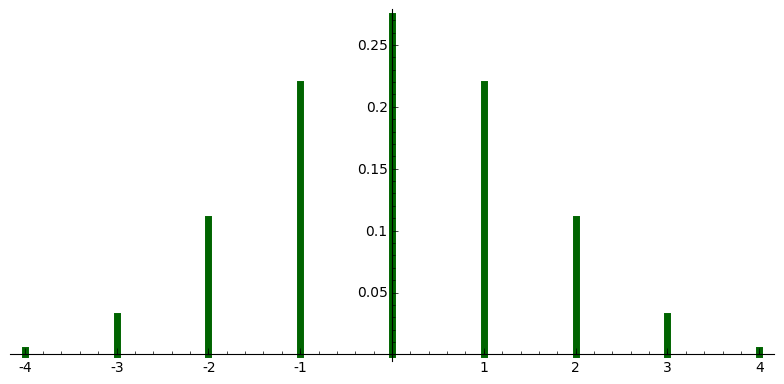
\includegraphics[width = 0.5\textwidth]{v8.png}
\caption{Probability density function of $\cV_{8}$}
\label{fig: v8}
\end{figure}


\begin{definition}
\label{def: modified distribution}
Let $k \geq 2$ be an even integer. Then a sample from the modified PLWE error distribution $P'_{m,k}$ is
\[
    e' = \sum_{i=0}^{n-1} e'_i \zeta_m^{i},
\]
where the coefficients $e'_i$ are sampled independently from $\cV_k$.
\end{definition}




\subsection{Bounding the Distance from Uniform}

We recall the definition and key properties of Fourier transform over finite fields.
Suppose $f$ is a real-valued function on $\bF_q$. The {\it Fourier transform} of $f$ is defined as
\[
    \widehat{f}(y) = \sum_{a \in \bF_q} f(a) \bar{\chi_y}(a),
\]
where $\chi_y(a) := e^{2 \pi i ay/q}$.

Let $u$ denote the probability density function of the uniform distribution over $\bF_q$, that is $u(a) = \frac{1}{q}$ for all $a \in \bF_q$. Let $\delta$ denote the characteristic function of the
one-point set $\{0\} \subseteq \bF_q$. Recall that the convolution of two functions $f,g: \bF_q \to \bR$ is
defined as $(f  \ast g ) (a) = \sum_{b \in \bF_q} f(a-b)g(b)$. We list without proof some basic properties of the Fourier transform.
\begin{enumerate}
\item $\widehat{\delta} = qu$; $\widehat{u} = \delta$.
\item $\widehat{f \ast g} = \widehat{f} \cdot \widehat{g}$.
\item $f(a) = \frac{1}{q} \sum_{y \in \bF_q} \widehat{f}(y)\chi_y(a)$ (the Fourier inversion formula).
%\item Plancherel's formula states that
%$||f||_2 = \frac{1}{q} ||\widehat{f}||_2$.
%\item $\widehat{f(a - \lambda)}(s) =  \bar{\chi_s(\lambda)} f(s)$.
\end{enumerate}

%Suppose $f,g$ are the probability density functions of two random variables $F,G$ with value in $\bF_q$. Let $h$ denote the density function of the sum $H =F+G$.
The following is a standard result.

\begin{lemma}
Suppose the random variables $F,G$ are independent random variables with values in $\bF_q$, having probability density functions $f$ and $g$.  Then $h =  f \ast g$.
In general, suppose $F_1, \cdots, F_n$ are mutually independent random variables in $\bF_q$, with probability density functions $f_1, \cdots, f_n$. Let $f$ denote the density function of the sum $F = \sum F_i$, then $f = f_1 \ast \cdots \ast f_n$.
\end{lemma}

%\begin{proof}
%We prove the first claim. For any $a \in \bF_q$,
%\begin{align*}
%\prob(F+G = a) &= \sum_{b \in \bF_q} \prob(F = a-b, G =b) \\
%& = \sum_{b \in \bF_q} \prob(F = a-b)\prob(G =b).  \qquad \mbox{(since $F,G$ are independent)} \\
%& = (f \ast g)(a).
%\end{align*}
%The general case follows from an induction on $n$.
%\qed \end{proof}

The Fourier transform of $\nu_k$ has a nice closed-form formula, as below.
\begin{lemma}
\label{lem: transform1}
For all even integers $k \geq 2$, $\widehat{\nu_k}(y)  = \cos \left(\frac{\pi y}{q}\right)^k.$
\end{lemma}

\begin{proof}  We have
\begin{align*}
2^k \cdot \widehat{\nu_k}(y) &= \sum_{m = -\frac{k}{2}}^{\frac{k}{2}} {k \choose m+\frac{k}{2}} e^{2\pi i ym/q}  \\
&= e^{-\pi i yk/q}\sum_{m = -\frac{k}{2}}^{\frac{k}{2}} {k \choose m+\frac{k}{2}} e^{2\pi i y(m+k/2)/q} \\
&= e^{-\pi i yk/q} \sum_{m' = 0}^{k} {k \choose m'} e^{2\pi i ym'/q} \\
& =  e^{-\pi i yk/q} (1+ e^{2 \pi i y/q})^k \\
& = (e^{-\pi i y/q} + e^{\pi i y/q})^k  \\
& = (2 \cos(\pi y/q))^k.
\end{align*}
Dividing both sides by $2^k$ gives the result.
\qed \end{proof}


Next, we concentrate on the reduced distributions $P_{m,\tau} \pmod{\fq}$ and $P'_{m,k} \pmod {\fq}$. Note that there is a one-to-one correspondence between primitive $m$-th roots of unity in $\bF_q$ and the prime ideals above $q$ in $\bQ(\zeta_m)$. Let $\alpha$ be the root corresponding to our choice of $\fq$. Then a sample from $P_{m, \tau} \pmod{\fq}$ (resp. $P'_{m,k} \pmod {\fq}$) is
of the form

$$ \sum_{i=0}^{n-1} \alpha^i e_i \pmod {q},$$

where $e_i$ are independent variables under the distribution $D_{\bZ,\tau}$ (resp. $\cV_k$). We use $e_\alpha$ and $e_\alpha'$ to denote their probability density functions. Then

\begin{lemma}
\label{lem: transform2}
\[
    \widehat{e_\alpha'}(y) = \prod_{i=1}^{n} \cos \left(\frac{ \alpha^i \pi y}{q} \right)^k.
\]
\end{lemma}

\begin{proof}
This follows directly from Lemma~\ref{lem: transform1} and the basic properties of Fourier transform.
\qed \end{proof}

Now we are able to bound the difference  using the Fourier inversion formula.

\begin{proposition} \label{prop: bound}
Let $f: \bF_q \to \bR$ be a function such that $\sum_{a \in \bF_q} f(a) = 1$. Then for all $a \in \bF_q$,
\begin{equation} \label{eq: secure}
    |f(a) -  1/q| \leq \frac{1}{q}  \sum_{y \in \bF_q, y \neq 0}  |\hat{f}(y)|.
\end{equation}
\end{proposition}

\begin{proof} For all $a \in \bF_q$,
\begin{align*}
    f(a) - 1/q &= f - u(a) \\
    & = \frac{1}{q} \sum_{y \in \bF_q} (\hat{f}(y) - \widehat{u}(y) )\chi_y(a) \\
& = \frac{1}{q} \sum_{y \in \bF_q} (\hat{f}(y)  - \delta(y) )\chi_y(a) \\
& = \frac{1}{q} \sum_{y \in \bF_q, y \neq 0} \hat{f}(y)  \chi_y(a).  \qquad \mbox{(since $\hat{f}(0) = 1$)}
\end{align*}
Now the result follows from taking absolute values on both sides, and noting that $|\chi_y(a)| \leq 1$ for all $a$ and all $y$.
\qed \end{proof}

Taking $f = e_\alpha$ or $f = e_\alpha'$ in Proposition~\ref{prop: bound}, we immediately obtain
\begin{theorem} \label{cor: stat dist}
The statistical distance between $e_\alpha$ and $u$ satisfies $$d(e_\alpha,u) \leq \frac{1}{2}  \sum_{y \in \bF_q, y \neq 0}  |\widehat{e_\alpha}(y)|.$$
Similarly,
\begin{equation} \label{distance}
d(e_\alpha',u) \leq \frac{1}{2}  \sum_{y \in \bF_q, y \neq 0}  |\widehat{e'_\alpha}(y)|.
\end{equation}
\end{theorem}



Now let $\epsilon'(m,q,k,\alpha)$ denote the right hand side of (\ref{distance}), i.e.,
\[
    \epsilon'(m,q,k, \alpha) = \frac{1}{2}\sum_{y \in \bF_q, y \neq 0} \prod_{i=0}^{n-1} \cos \left(\frac{ \alpha^i \pi y}{q} \right)^k.
\]
To take into account all prime ideals above $q$, we let $\alpha$ run through all primitive $m$-th roots of unity in $\bF_q$ and define
$$\epsilon'(m,q,k) := \max \{\epsilon'(m,q,k,\alpha): \alpha \mbox{ has order } m \mbox{ in } \bF_q\}.$$
If $\epsilon'(m,q,k)$ is negligibly small, the distribution $P'_{m,k} \pmod {\fq}$ will be computationally indistinguishable from uniform.

We can run the same analysis for the PLWE distribution, with the only difference being that there is no obvious closed-form formula for the density function $d$  of $D_{\bZ,\tau} \pmod{q}$. Nonetheless, we could numerically approximate this probability density function, using the formula
\[
        d(a)  = \frac{\displaystyle{\sum_{\substack{z \in \bZ\\ z \equiv a\bmod{q}}} e^{-|z|^2/2\tau}}}{\displaystyle{\sum_{z \in \bZ} e^{-|z|^2/2\tau}}}, \quad \forall a \in \bF_q.
\]
Since the sums in the definition of $d(a)$ converge rapidly, we could obtain good approximations of $d$ by truncating the sums and then evaluating. Then we compute numerically the Fourier transform $\hat{d}$, and obtain
\[
    \widehat{e_\alpha}(y) = \prod_{i=0}^{n-1} \hat{d}(\alpha^i y)
\]
Finally, we compute $\epsilon(m,q,\tau) = \frac{1}{2} \sum_{y \in \bF_q, y \neq 0} \prod_{i=0}^{n-1} \widehat{d}(\alpha^i y)$. Then $\epsilon(m,q,\tau)$ is an upper bound of the statistical distance  between the distribution $e_\alpha$ and the uniform distribution over $\bF_q$.

\subsection{Numerical Distance from Uniform}

We have computed $\epsilon'(m,q,k)$ and $\epsilon(m,q,k)$ for various choices of parameters.  Smaller values imply that the error distribution looks uniform when transfered to $R/\mathfrak{q}$, rendering the instance of RLWE invulnerable to the attacks suggested in this paper.

The following is a table of data. Noe that we chose $k = 2$ and $\tau = 1$. For each instance in the table, we also  generated the RLWE samples (where we fixed $\sigma_0 = 1$) and ran the chi-square attack using the confidence level $\alpha = 0.99$. The column labeled ``$\chi^2$'' contains the $\chi^2$ values we obtained, and the column labeled ``uniform?'' indicates whether the reduced errors are uniform. We can see from data how the practical situation agrees with our analysis on the approximated distributions.


\begin{table}[H]
\caption{Values of $\epsilon'(m,q,2)$ and $\epsilon(m,q,1)$ and the $\chi^2$ values}
\label{tab: deg1}
\begin{center}
\begin{tabular}{c|c|c|c|c|c|c}
$m$ & $n$ & $q$ & $-[\log_2(\epsilon'(m,q, 2))]$ & $-[\log_2(\epsilon(m,q, 1))]$ & $\chi^2$ & uniform? \\
\hline
96 & 32 & 193 & $35$ & 38 & 231.6 & yes \\
55 & 40 & 331  & $44$ & 51 & 308.8 & yes \\
160 & 64 & 641 & 55 & 79& 658.0 & yes \\
101 & 100 & 1213 & $177$ & 203 & 1254.4 & yes \\
%145 & 112  &19163 & $176$  & 176\\
244 & 120 & 1709 & 230 & 248 & 1721.2 & yes \\
256 & 128 & 3329 & $194$ & 253 & 3350.0 & yes \\
%256 & 128 & 14081 & $208$ & 240 \\
197 & 196 & 3547 & $337$ & 410 & 3475.2 & yes \\
512 & 256 &10753 & 431 & 511 &  & yes\\
% 512 & 256 &19457 & 414 & 512 &
\end{tabular}
\end{center}
\end{table}

The data in Table~\ref{tab: deg1} suggests that for $n \geq 100$ and $q$ of polynomial size in $n$, the statistical distance between $P'_{m,k} \pmod{\fq}$ (or $P_{m,\tau} \pmod{\fq})$ and the uniform distribution is negligibly small. Also, note that we fixed $k= 2$ and $\tau = 1$, and the $\epsilon$ values becomes even smaller when $k$ increases.


It is possible to generalize our discussion in this section to primes of arbitrary residue degree, in which case the Fourier analysis will be performed over the corresponding extension field. The only change in the definitions would be $\chi_y(a) = e^{ \frac{2 \pi i Tr(a y)}{q}}$. Similarly, we have
\[
    \widehat{e'_\alpha}(y) = \prod_{i=1}^{n} \cos \left(\frac{ \pi Tr(\alpha^i y) }{q} \right)^k.
\]
Table~\ref{tab: deg2} contains some data for primes of degree two.

\begin{table}[H]
\caption{Values of $\epsilon'(m,q,2)$ for primes of degree two}
\begin{center}
\begin{tabular}{c|c|c} \label{tab: deg2}
$m$ & $q$ & $-[\log_2(\epsilon'(m,q,2))]$ \\
\hline
53 & 211 & 61 \\
55 & 109 & 48 \\
63 & 881 & 33 \\
%64 & 127 & 37 \\
%64 & 191 & 35 \\
64 & 383 & 31 \\
512 & 257 & 263
\end{tabular}
\end{center}
\end{table}

\subsection{Heuristics}

There is a heuristic argument as to why one expects $\epsilon'(m,q,k,\alpha)$ to be small. Each term in the summand is a product of form $\prod_{i=0}^{n-1} \cos \left(\frac{ \alpha^i \pi y}{q} \right)^k$. For each $0 \neq y \in \bF_q$, if one assumes the elements $\alpha^i$ are distinct and uniformly distributed in $\bF_q$, it is very likely that $\alpha^i y$ is close to $q/2$ for at least some values of $i$, making the product of cosines small.

\bibliographystyle{splncs}
\bibliography{galois-rlwe}

\end{document}
